\section{Project Activities}\label{sec:activities}

\subsection{Division of tasks}
\Cref{tab:team} lists who did what. Each member also wrote the report section on
their own part.

\begin{table}[t]
\centering
\caption{Team members and responsibilities}\label{tab:team}
\begin{tabularx}{\columnwidth}{@{}>{\raggedright\arraybackslash}p{0.22\columnwidth}>{\raggedright\arraybackslash}X@{}}
\toprule
Member & Responsibilities \\
\midrule
Chen Jinxian & Team lead; cluster infrastructure: Docker image, Compose file, Hadoop/YARN configuration, resource caps; report editing \\[2pt]
Yang Ye & Algorithms: mapper, reducer/combiner, PySpark jobs, serial baseline, correctness checks \\[2pt]
Gong Pengxiang & Data and benchmarking: data preparation, benchmark and cache-experiment scripts, figures \\[2pt]
Ma Jiajun & Cloud deployment on Azure, cloud measurements, demonstration video \\
\bottomrule
\end{tabularx}
\end{table}

\textbf{Timeline.} 23~Nov 2026: Docker image built and smoke test with two workers
passed. 24~Nov: data tiers prepared, Azure cluster deployed and the 225 cloud runs
completed; local benchmark started. 25~Nov: local benchmark (561 runs) and cache
experiment (48 runs) completed, figures and first report draft. December: report
revision and demonstration video.

\subsection{Installation process}
All software runs inside Docker containers~\cite{merkel2014docker}, so the host only needs Docker.
\begin{enumerate}
  \item \textbf{Host preparation.} Enable WSL\,2 on Windows~11 and install Docker
        Desktop with the WSL\,2 back end. Raise the memory available to the WSL\,2 VM
        in \texttt{.wslconfig} to 26\,GB, because the default limit (half of the
        host RAM) is too small for a master plus four 5\,GB workers.
  \item \textbf{Cluster image.} \texttt{cluster/Dockerfile} starts from Eclipse
        Temurin JDK\,11 on Ubuntu 22.04, adds Python~3, and unpacks Hadoop 3.4.1 and
        Spark 3.5.5 (pre-built for Hadoop~3). The Hadoop XML files and
        \texttt{spark-defaults.conf} are copied in, and all daemons run as an
        unprivileged \texttt{hadoop} user.
  \item \textbf{Roles.} The same image starts as \emph{master} (HDFS NameNode~\cite{shvachko2010hdfs}, YARN
        ResourceManager~\cite{vavilapalli2013yarn}, MapReduce JobHistory server) or \emph{worker} (DataNode and
        NodeManager), selected by \texttt{entrypoint.sh}.
  \item \textbf{Cluster start.} \texttt{scripts/cluster.sh up N} recreates the
        cluster with $N$ workers, waits until $N$ DataNodes and $N$ NodeManagers have
        registered, and uploads the Spark jars to HDFS once so that Spark jobs do not
        re-upload them on every submission.
  \item \textbf{Smoke test.} With two workers and tier S, all five engines and three
        jobs ran and their outputs matched. The web interfaces of HDFS (port 9870),
        YARN (8088) and the JobHistory server (19888) show the live nodes and every
        job; \cref{fig:yarn} shows the four-worker cluster.
\end{enumerate}

\begin{figure*}[t]
\centering
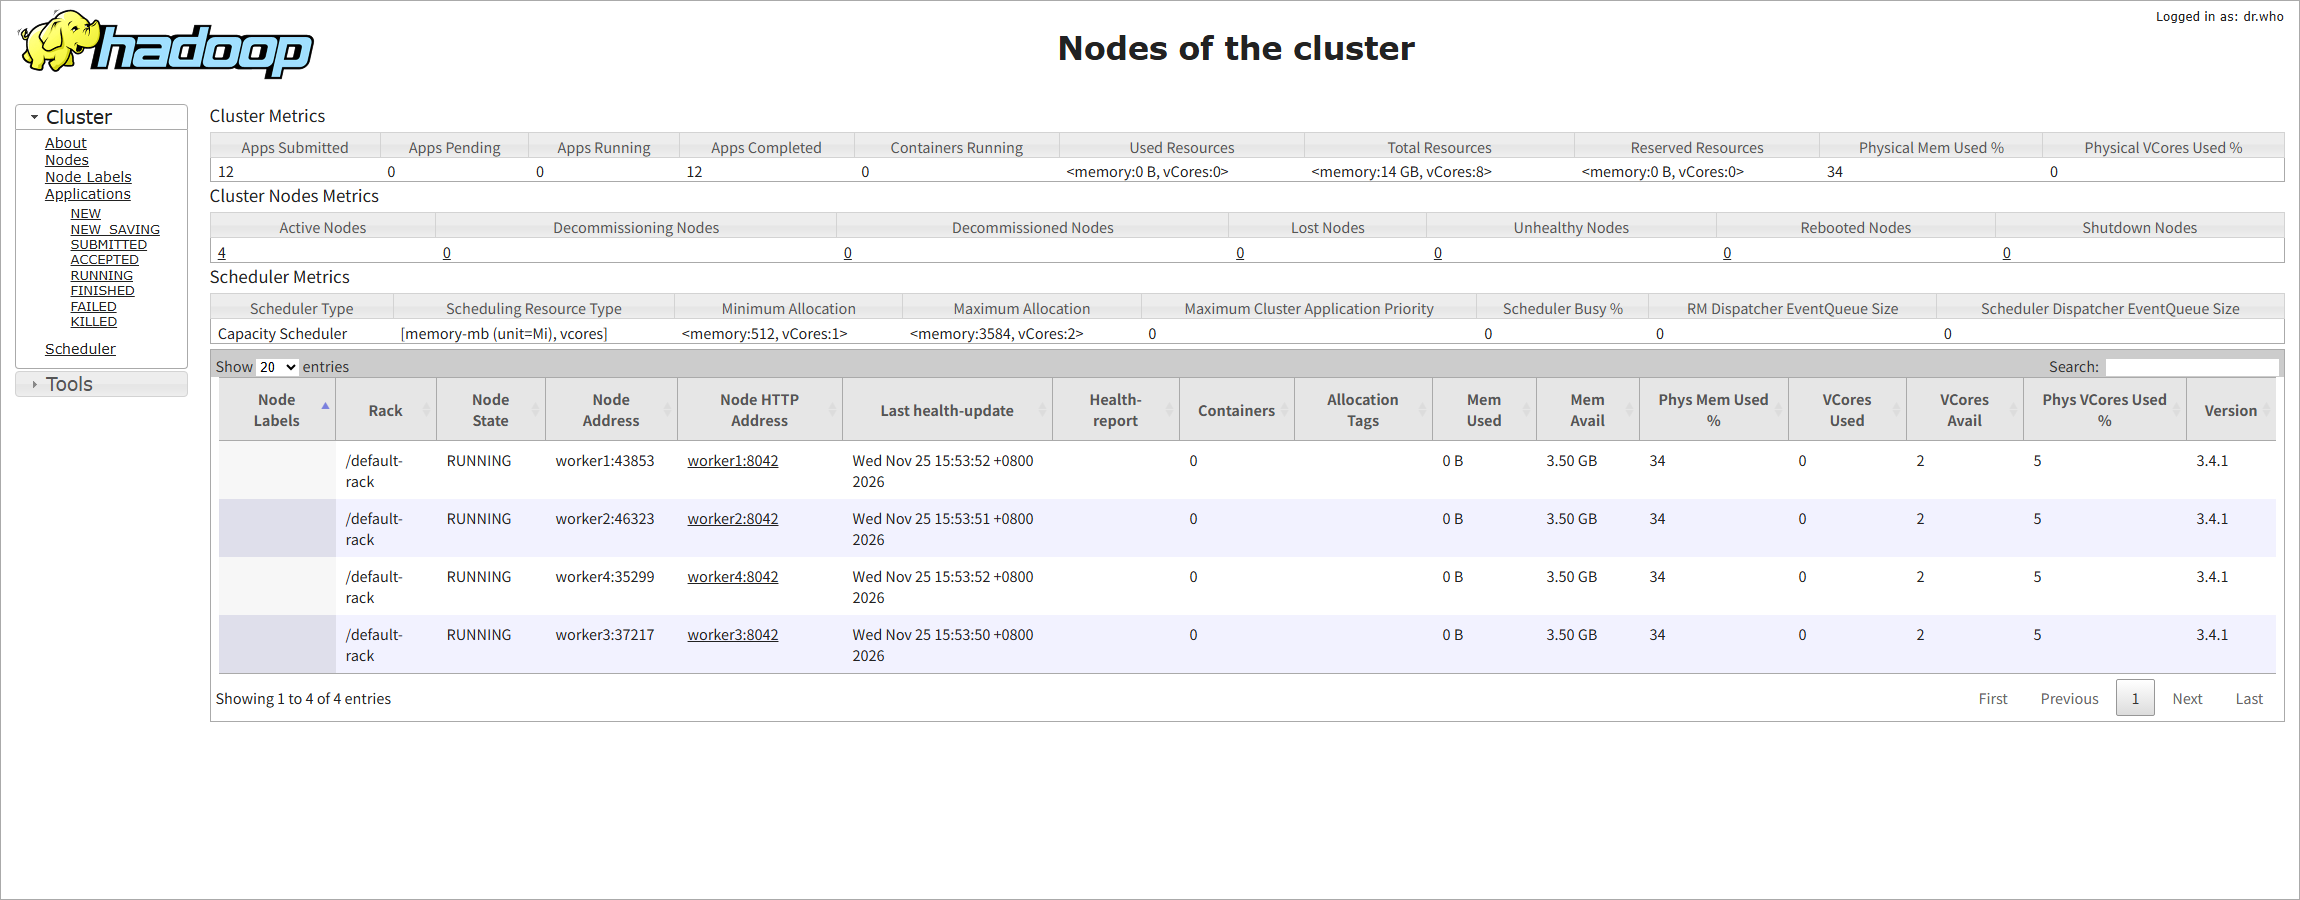
\includegraphics[width=\textwidth,trim=200 150 0 95,clip]{figures/yarn_nodes.png}
\caption{YARN ResourceManager web interface (port 8088) of the local cluster with four
workers: four active NodeManagers with 3.5\,GB and 2 vcores each (14\,GB and 8 vcores in
total), after the 12 jobs of the cache experiment on this cluster.}\label{fig:yarn}
\end{figure*}

\textbf{Problems and solutions.} (1)~Git Bash rewrites arguments such as
\texttt{/opt/scripts} into Windows paths before passing them to \texttt{docker}; the
scripts set \texttt{MSYS\_NO\_PATHCONV=1}. (2)~A separate \texttt{chown} layer in the
Dockerfile duplicated the Hadoop and Spark files and made the image 6.2\,GB; changing
ownership in the same layer as the extraction reduced it to 3.9\,GB. (3)~Without
explicit limits, one container could use all 20 host threads, so ``one worker'' was
not one machine; we cap CPU and memory per container and make YARN advertise the same
amounts. (4)~On Azure, a VM resolved its own name to an IPv6 link-local address that
the Hadoop daemons could not use; we pin all names to the private IPv4 addresses.
(5)~The full local sweep took many hours and was interrupted several times by restarts
of the WSL\,2 VM, Docker Desktop and Windows; \texttt{run\_benchmark.sh} therefore records every run and
skips completed ones when restarted.
